En esta sección se detallarán los casos de uso pertenecientes al subsistema de gestión de eventos. La figura \ref{fig:casos_uso_subsistema_eventos} muestra el diagrama de casos de uso de dicho subsistema.

\begin{figure}[h]
\centering
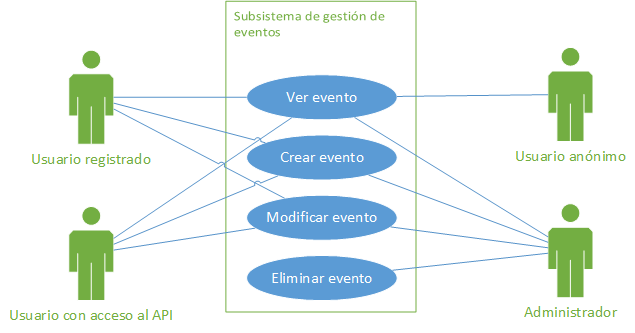
\includegraphics[width=\textwidth]{casos_uso_eventos}
\caption{Diagrama de casos de uso del subsistema de gestión de eventos}
\label{fig:casos_uso_subsistema_eventos}
\end{figure}


\subsubsection{Caso de uso ``ver evento''}
\begin{description}
\item[Descripción] Un usuario quiere ver el contenido de un evento.
\item[Actores] Cualquier usuario registrado o no en el sistema.
\item[Escenario principal] 	\hfill
							\begin{enumerate}
							\item El usuario accede a la vista de eventos.
							\item Una vez en la vista de eventos, elige el evento del que quiere ver sus contenidos.
							\item Pulsa en el título del evento que quiere ver en detalle.
							\item El sistema carga la vista del evento mostrando todos sus detalles.
							\end{enumerate}
\end{description}


\subsubsection{Caso de uso ``crear evento''}
\begin{description}
\item[Descripción]  Un usuario quiere añadir un nuevo evento al sistema.
\item[Actores]  Administrador, usuario registrado o usuario con capacidad de acceso al API.
\item[Precondiciones] Haber iniciado sesión en el sistema.
\item[Escenario principal]  \hfill
							\begin{enumerate}
							\item El usuario accede a la vista de los eventos.
							\item Una vez en la vista de eventos pulsa el botón correspondiente para crear un evento nuevo.
							\item Rellena el formulario con los datos requeridos.
							\item Si lo desea también rellena la información opcional del formulario.
							\item El usuario pulsa el botón guardar, y el sistema crea el nuevo evento.
							\end{enumerate}
\item[Escenario alternativo 1] No se han rellenado todos los campos requeridos.
							\begin{enumerate}
							\item El usuario no ha rellenado todos los campos requeridos para crear un nuevo evento.
							\item El sistema notificará al usuario de su error y no creará el nuevo evento.
							\item Se continuará desde el punto 3 del escenario principal.
							\end{enumerate}
\end{description}


\subsubsection{Caso de uso ``modificar evento''}
\begin{description}
\item[Descripción]  Un usuario quiere modificar un evento del sistema.
\item[Actores]  Administrador, usuario registrado o usuario con capacidad de acceso al API.
\item[Precondiciones]  Haber iniciado sesión en el sistema.
\item[Escenario principal]	\hfill
							\begin{enumerate}
							\item El usuario accede a la vista de los eventos..
							\item Una vez en la vista de eventos localiza el evento que quiere modificar.
							\item Cuando ha accedido al evento pulsa el botón correspondiente para modificar su contenido.
							\item Rellena toda la información requerida en el formulario.
							\item Si lo desea también rellena la información opcional del formulario.
							\item El usuario pulas el botón guardar y el sistema modifica la información del evento.
							\end{enumerate}
\item[Escenario alternativo 1] No se han rellenado todos los campos requeridos.
							\begin{enumerate}
							\item El usuario no ha rellenado todos los campos requeridos para modificar el evento.
							\item El sistema notificará al usuario de su error y no modificará los datos del evento.
							\item Se continuará desde el punto 4 del escenario principal.
							\end{enumerate}
\end{description}


\subsubsection{Caso de uso ``eliminar evento''}
\begin{description}
\item[Descripción]  Un administrador quiere eliminar un evento del sistema.
\item[Actores] El administrador del sistema.
\item[Precondiciones]  Haber iniciado sesión en el sistema.
\item[Escenario principal]	\hfill
							\begin{enumerate}
							\item El administrador accede a la vista de administración.
							\item Localiza el evento que desea eliminar y pulsa el botón correspondiente.
							\item El evento será eliminado del sistema.
							\end{enumerate}
\end{description}